
\chapter{راهنمای استفاده}


در این بخش، راهنمای استفاده از بخش‌های مختلف سیستم برنامه‌ریزی برای منابع سازمان شرح داده شده است.

\renewcommand*\contentsname{فهرست راهنمای استفاده}
\localtableofcontents

\newpage
\section{تعارف اولیه}
\subsection{انواع سطوح دسترسی}
سیستم برنامه‌ریزی بر اساس سه سطح دسترسی اصلی کار می‌کند. این سطوح عبارتند از:
\begin{enumerate}
	\item سطح دسترسی ویژه مدیران ارشد
	\item سطح دسترسی ویژه مدیران میانی
	\item سطح دسترسی ویژه کارمندان معمولی \\
\end{enumerate}


عملیاتی که انجام آن‌ها منوط به داشتن مجوز است، عبارتند از:
\begin{enumerate}
	\item افزودن واحد
	\item دریافت گزارش
	\item جستجو
	\item دریافت مشخصات منبع
	\item افزودن و حذف منبع
	\item افزودن و حذف نیازمندی
	\item افزودن  پروژه
	\item افزودن و حذف سیستم و ماژول
	\item تغییر سطح دسترسی
	\item تایید ثبت‌نام کاربر دیگر
\end{enumerate}

این سطوح دسترسی قابل تغییر هستند که در بخش‌های جلوتر توضیح داده خواهد شد.

\subsection{انواع منابع}
سیستم برنامه‌ریزی در حال حاضر از ۴ نوع منبع پشتیبانی می‌کند که عبارتند از: منبع فیزیکی، منبع انسانی، منبع اطلاعاتی و منبع مالی. می‌توان به سیستم برنامه‌ریزی منبع اضافه کرد، آن‌ها را ویرایش کرد و گزارش‌هایی از آن‌ها تهیه نمود.

\newpage
\section{ورود به سیستم برنامه‌ریزی}
پس از اجرای نرم‌افزار، نخستین صفحه‌ای که کاربر با آن مواجه خواهد شد، صفحه‌ی ورود به سیستم است. در این صفحه با وارد کردن شناسه‌ی کاربری و رمز عبور و سپس فشردن دکمه‌ی ورود  (۱) می‌توان وارد سیستم شد. شناسه‌ی کاربری یک عدد ۶ رقمی است که باید از فرمدار دریافت شود. وقایعی که ممکن است ورود به سیستم برنامه‌ریزی را با خطا مواجه کنند عبارتند از: خطا در شناسه‌ی کاربری و/یا رمز عبور، عدم تایید ثبت‌نام کاربر.
	\begin{figure}[H]
		\centering
		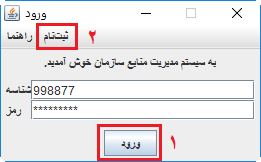
\includegraphics[scale=0.8]{img/manual/login}
		\caption{ورود به سیستم برنامه‌ریزی}
	\end{figure}

هنگامی که ورود موفقیت‌آمیز باشد، به صفحه‌ی اصلی کاربری هدایت خواهید شد. در صورتی که کاربر فاقد شناسه‌ی کاربری است، با انتخاب گزینه‌ی «ثبت‌نام»   (۲) می‌تواند در سیستم برنامه‌ریزی ثبت‌نام کند تا پس از تایید شدن، وارد سیستم شود.

صفحه‌ی ثبت‌نام در شکل زیر قابل مشاهده است. پس از اینکه جعبه‌های اطلاعات (۱) را پر کردید، گزینه‌ی ثبت‌نام (۲) را انتخاب کنید تا اطلاعات شما در سیستم برنامه‌ریزی ثبت گردد. شناسه‌ی کاربری (کد پرسنلی) شما به صورت خودکار و توسط سیستم تولید می‌گردد که می‌توانید با مراجعه به فرمدار
\LTRfootnote{Administrator}
از آن مطلع شوید.

	\begin{figure}[H]
		\centering
		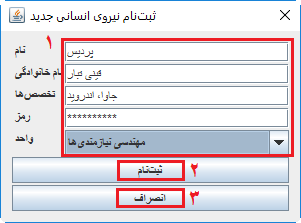
\includegraphics[scale=0.8]{img/manual/register}
		\caption{ثبت‌نام در سیستم برنامه‌ریزی}
	\end{figure}


\newpage
\section{صفحه اصلی کاربری}
این صفحه که پس از ورود موفقیت‌آمیز به سیستم برنامه‌ریزی به آن هدایت خواهید شد، شامل یک پیام خوشامدگویی  (۱) و  همچنین یک منوی اصلی  (۲)است. با توجه به سطح دسترسی کاربر وارد شده، هر کدام از زیرمنوها شامل تعدادی گزینه است.

	\begin{figure}[H]
		\centering
		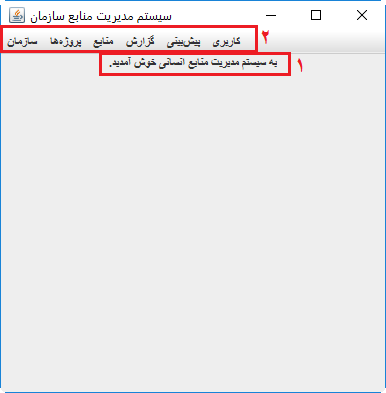
\includegraphics[scale=0.7]{img/manual/main}
		\caption{صفحه‌ی اصلی}
	\end{figure}

در بخش‌های بعدی، عملیاتی که می‌توان با انتخاب هر کدام از گزینه‌ها انجام داد شرح داده شده است.

\newpage
\section{زیرمنوی سازمان}
برای انجام عملیاتی که به کل سازمان مربوط می‌شوند، به این زیرمنو مراجعه کنید. در این بخش می‌توانید به برزش واحدها یا نیازمندی‌ها بپردازید.
	\begin{figure}[H]
		\centering
		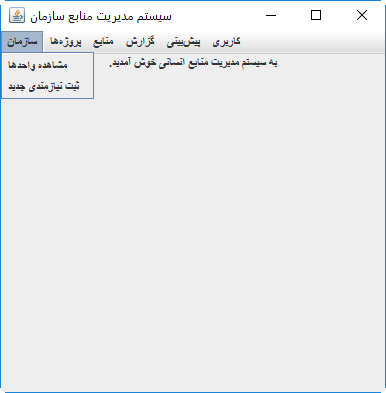
\includegraphics[scale=0.7]{img/manual/orgSubmenu}
		\caption{زیرمنوی سازمان}
	\end{figure}

\subsection{مشاهده واحدها}
با انتخاب گزینه‌ی مشاهده‌ی واحدها به صفحه‌ی زیر هدایت می‌شوید.
	\begin{figure}[H]
		\centering
		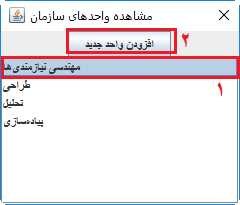
\includegraphics[scale=0.9]{img/manual/viewUnits}
		\caption{مشاهده واحدها}
	\end{figure}
همان‌طور که در شکل بالا مشاهده می‌کنید، فهرستی از واحدهای سازمان نمایش داده می‌شود. (۲: یک نمونه واحد) در این صفحه با فشردن دکمه‌ی افزودن واحد (۲) به صفحه‌ای جهت اضافه کردن واحد به سازمان هدایت می‌شوید که در شکل زیر قایل مشاهده است.
	\begin{figure}[H]
		\centering
		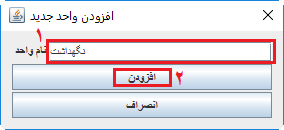
\includegraphics[scale=0.8]{img/manual/addUnit}
		\caption{افزودن واحد}
	\end{figure}
در این صفحه ابتدا با وارد کردن نام واحد (۱) و سپس فشردن دکمه‌ی افزودن (۲) واحد به سیستم برنامه‌ریزی اضافه خواهد شد.

\subsection{ثبت نیازمندی جدید}
({\color{red} تکمیل نشده است. })


\newpage
\section{زیرمنوی پروژه‌ها}
این بخش برای هدایت شدن به تمامی عملیات مربوط به پروژه‌های سازمان است.
	\begin{figure}[H]
		\centering
		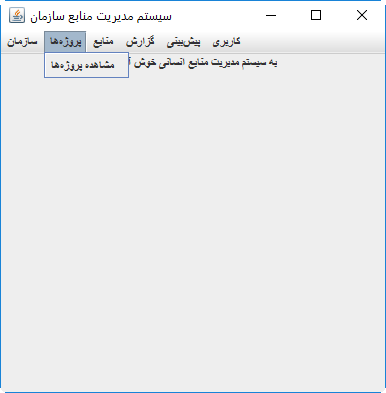
\includegraphics[scale=0.7]{img/manual/prjSubmenu}
		\caption{زیرمنوی پروژه‌ها}
	\end{figure}
	
\subsection{مشاهده پروژه‌ها}
با انتخاب گزینه‌ی مشاهده‌ی پروژه‌ها، به صفحه‌ی زیر هدایت می‌شوید:
	\begin{figure}[H]
		\centering
		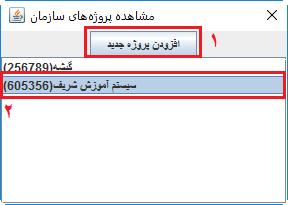
\includegraphics[scale=0.7]{img/manual/viewProjects}
		\caption{مشاهده پروژه‌ها}
	\end{figure}
در این صفحه با فشردن دکمه‌ی افزودن پروژه‌ی جدید (۱) به صفحه‌ای جهت ورود اطلاعات پروژه وارد می‌شوید. (شکل 
\ref{f1}
 )
همچنین، با دوبار کلیک کردن بر روی هر کدام از پروژه‌ها (۲) به صفحه‌ای هدایت‌ می‌شوید که امکان مشاهده و ویرایش پروژه‌ی انتخاب شده را در اختیار شما می‌گذارد. (شکل  
\ref{f2}
 )


\subsubsection{افزودن پروژه جدید}

در صفحه‌ی افزودن پروژه‌ی جدید، (شکل
\ref{f1}
)
ابتدا نام پروژه (۱) را وارد می نمایید. سپس می‌توانید  یک یا چند واحد درگیر (۲) را انتخاب کنید. به این صورت که بر روی صفحه کلید کامپیوتر خود، دکمه‌ی Ctrl را نگه داشته و روی واحدهای مدنظرتان کلیک می‌کنید. برای حذف موردی که برگزیده‌اید، در هنگام نگه‌داشتن Ctrl ، دوباره روی آن کلیک نمایید. سپس گزینه‌ی افزودن (۳) را فشار دهید تا پروژه جدید به سیستم اضافه گردد.

\begin{figure}[H]
	\centering
	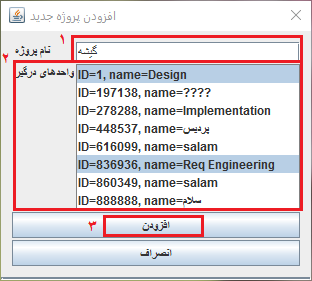
\includegraphics[scale=0.8]{img/manual/addProject}
	\caption{افزودن پروژه جدید}
	\label{f1}
\end{figure}

\subsubsection{مشاهده پروژه}
صفحه‌ي مشاهده‌ی مشخصات پروژه (شکل
\ref{f2}
)
دارای چند بخش اصلی است. در بخش سمت راست صفحه، اطلاعات ابتدایی پروژه (۱) مشاهده می‌شود. در بخش میانی (۲) تکنولوژی‌ها و واحدهای درگیر در پروژه قابل مشاهده هستند و در بخش سمت چپ (۵) ساختار سلسله‌مراتبی سیستم‌ها و ماژول‌های پروژه قابل مشاهده است. با کلیک بر روی علامت کلیدی که در سمت چپ هر سیستم وجود دارد، می‌توان اطلاعات آن را گسترش یا کاهش داد. در صورتی که در این بخش کلید سمت راست موشواره را فشار دهید، یک منوی جدید باز می‌شود که از طریق آن می‌توان به پروژه سیستم و ماژول اضافه کرد یا اینکه به برزش تغییرات ماژول پرداخت. (شکل
\ref{f3}
) \\
برای مشاهده اطلاعات دیگر پروژه (منابع و نیازمندی‌ها) از بخش‌های ۳ و ۴ استفاده نمایید.
\begin{figure}[H]
	\centering
	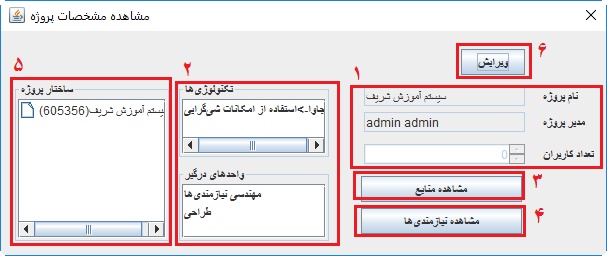
\includegraphics[scale=0.8]{img/manual/projectAttr}
	\caption{مشاهده پروژه}
	\label{f2}
	\end{figure}	

\subsubsection{افزودن منبع به پروژه}
هنگامی که بر روی بخش ۳ در شکل
\ref{f2}
کلیک کنید، صفحه‌ی مطابق زیر برای شما باز می‌گردد که در آن می‌توان منابع پروژه را مشاهده کرد. همچنین، با دکمه‌ی افزودن منبع (۱) می‌توانید یک منبع به پروژه بیفزایید.

\begin{figure}[H]
	\centering
	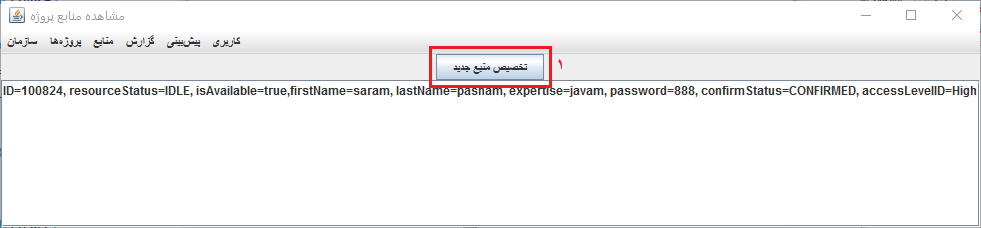
\includegraphics[scale=0.5]{img/manual/addResToProject}
	\caption{افزودن منبع به پروژه}
	\label{f4}
\end{figure}	


\subsubsection{افزودن نیازمندی به پروژه}
({\color{red}  تکمیل نشده است. })

هنگامی که بر روی بخش 4 در شکل
\ref{f2}
کلیک کنید، صفحه‌ی مطابق زیر برای شما باز می‌گردد که در آن می‌توان نیازمندی‌های پروژه را مشاهده کرد. همچنین، با دکمه‌ی افزودن نیازمندی (۱) می‌توانید یک نیازمندی جدید به پروژه بیفزایید.

\begin{figure}[H]
	\centering
%	\includegraphics[scale=0.7]{img/manual/addReqToProject}
	\caption{افزودن نیازمندی به پروژه}
	\label{f5}
\end{figure}


\subsubsection{ویرایش پروژه}
هنگامی که بر روی بخش ۶ در شکل
\ref{f2}
کلیک کنید، صفحه‌ی مطابق زیر برای شما باز می‌گردد که در آن می‌توان  به ویرایش اطلاعات پروژه پرداخت.

\begin{figure}[H]
	\centering
	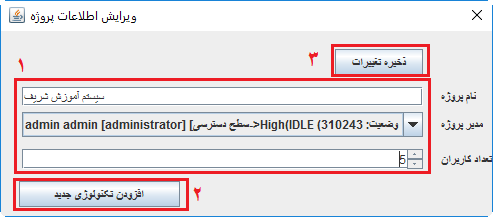
\includegraphics[scale=0.5]{img/manual/editProject}
	\caption{ویرایش پروژه}
	\label{f6}
\end{figure}
در بخش ۱ می‌توان اطلاعات ابتدایی پروژه را تغییر داد. توجه داشته باشید که در جعبه‌ی متنی تعداد کاربران، تنها عدد صحیح پذیرفته است و در غیر این صورت با پیغام خطا مواجه خواهید شد.  برای ذخیره شدن تغییرات گزینه‌ی ذخیره تغییرات (۳) را بفشارید. با کلیک بر روی افزودن تکنولوژی جدید (۲) صفحه‌ی جدیدی باز می‌شود که در زیر قابل مشاهده است.
\begin{figure}[H]
	\centering
	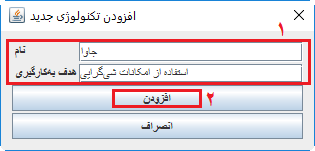
\includegraphics[scale=0.7]{img/manual/addTech}
	\caption{ افزودن تکنولوژی جدید}
	\label{f7}
\end{figure}
در این صفحه با وارد کردن نام و هدف به کار تکنولوژی (۱) و فشردن گزینه‌ی افزودن (۲) تکنولوژی به پروژه اضافه خواهد شد و نیازی نیست که دکمه‌ی ذخیره تغییرات صفحه‌ی ویرایش پروژه را (شکل
\ref{f6}
)
را بفشارید.

\newpage
\section{زیرمنوی منابع}
این زیرمنو شامل عملیاتی که سیستم برنامه‌ریزی برای کار با منابع در اختیار کاربر می‌گذارد.

	\begin{figure}[H]
		\centering
		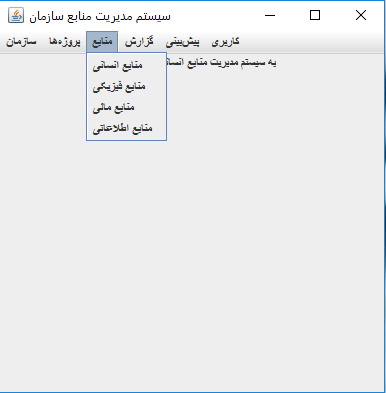
\includegraphics[scale=0.7]{img/manual/resSubmenu}
		\caption{زیرمنوی منابع}
	\end{figure}

\subsection{منابع انسانی}
این بخش شامل فهرست همه‌ی منابع انسانی سازمان است.
	\begin{figure}[H]
		\centering
		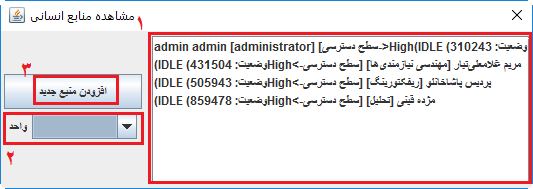
\includegraphics[scale=0.5]{img/manual/hRess}
		\caption{مشاهده منابع انسانی}
		\label{f10}
	\end{figure}

در ابتدا که صفحه باز می‌گردد، همه‌ی منابع انسانی سازمان نمایش داده می‌شوند. اما با استفاده از بخش ۲ می‌توان واحد را مشخص کرد تا تنها منابع مربوط به آن واحد نمایش داده شود. در صورتی که گزینه‌ی اول این کشو انتخاب گردد، منابع انسانی همه‌ی واحدها نشان داده می‌شود.
\subsubsection{افزودن منبع انسانی}
برای افزودن یک منبع انسانی جدید، روی افزودن منبع جدید (۳) کلیک کنید تا صفحه‌ای مطابق زیر برای شما باز گردد:
	\begin{figure}[H]
		\centering
		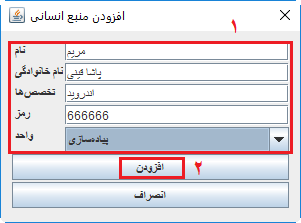
\includegraphics[scale=0.9]{img/manual/addHRess}
		\caption{افزودن منبع انسانی}
	\end{figure}
پس از وارد کردن اطلاعات منبع در بخش ۱ و فشردن دکمه‌ی افزودن (۲) یک منبع انسانی جدید به واحد مربوطه اضافه خواهد شد.

\subsubsection{مشاهده/ویرایش منبع انسانی}
برای مشاهده یا ویرایش منبع انسانی مورد نظر، در صفحه‌ی شکل
\ref{f10}
 روی منبع موردنظر دوبار کلیک کنید تا صفحه‌ای مطابق زیر برای شما باز گردد.

	\begin{figure}[H]
		\centering
		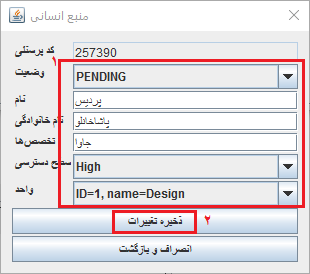
\includegraphics[scale=0.9]{img/manual/editHRess}
		\caption{مشاهده/ویرایش منبع انسانی}
		\label{f20}
	\end{figure} 
در این صفحه مشخصات منبع انتخاب شده نمایش داده می‌شود و اگر بخواهید می‌توانید هرکدام از فقره اطلاعات را تغییر دهید و با فشردن گزینه‌ی ذخیره تغییرات (۲) تغییرات مدنظر را به منبع اعمال نمایید.

\subsubsection{تعیین/تغییر سطح دسترسی کاربر دیگر}
همان‌طور که در شکل
\ref{f20}
قابل مشاهده است، امکان تعیین/تغییر سطح دسترسی کاربر دیگر، در صورت داشتن اجازه‌ی مربوطه، از طریق بخش ویرایش مشخصات منبع انسانی انجام می‌شود. به این صورت که روی بخش سطح دسترسی کلیک کرده و سطح مورد نظر را انتخاب می‌نمایید.

\subsubsection{تایید ثبت‌نام کاربر دیگر}
همان‌طور که در شکل
\ref{f20}
قابل مشاهده است، امکان تایید ثبت‌نام کاربر دیگر، در صورت داشتن اجازه‌ی مربوطه، از طریق بخش ویرایش مشخصات منبع انسانی انجام می‌شود. به این صورت که بر روی بخش وضعیت کلیک کرده و مورد «تایید شده یا Confirmed» را انتخاب می‌نمایید.


\subsection{منابع فیزیکی، مالی و اطلاعاتی}
عملیاتی که برای این سه منبع در اختیار کاربر قرار می‌گیرد، مشابه عملیاتی است که برای منابع انسانی در بخش قبل شرح داده شد (جز در موارد تایید ثبت‌نام و سطح دسترسی).   لذا از تکرار این موارد مشابه خودداری می‌کنیم.

\newpage
\section{زیرمنوی گزارش}
در این بخش می‌توان همه‌ي انواع گزارش‌هایی را که مدنظر نیروهای انسانی سازمان است تهیه نمود.
	\begin{figure}[H]
		\centering
		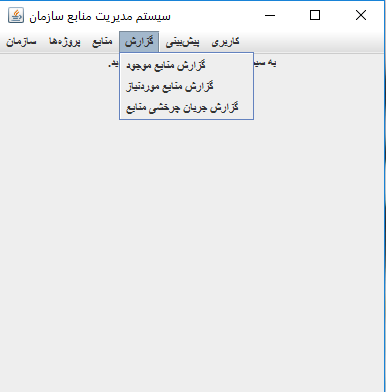
\includegraphics[scale=0.7]{img/manual/repSubmenu}
		\caption{زیرمنوی گزارش}
	\end{figure}
	
\subsection{گزارش منابع موجود}
 این صفحه، همه‌ی منابعی را که در سازمان موجود است و در حال حاضر در هیچ یک از پروژه‌ها استفاده نمی‌شود نمایش می‌دهد. به عبارت دیگر این گزارش نشان می‌دهد که از هر یک از انواع منابع موجود به چه میزان و در کدام قسمت از سازمان موجود است.
	\begin{figure}[H]
		\centering
		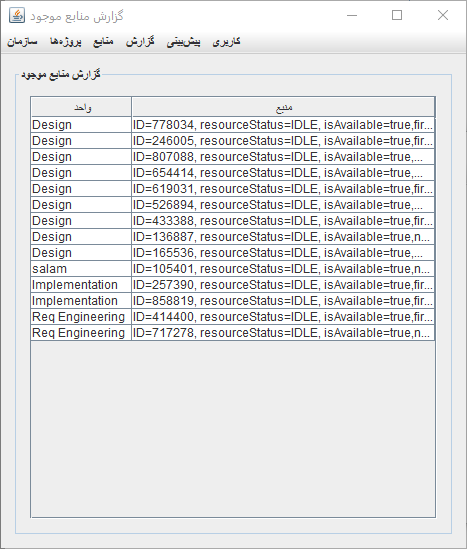
\includegraphics[scale=0.6]{img/manual/availRep}
		\caption{گزارش منابع موجود}
	\end{figure}


\subsection{گزارش منابع موردنیاز}
این گزارش نشان می‌دهد که در هر یک از پروژه‌ها چه منابعی مورد نیاز  (بوده) است.\\
برای دریافت این گزارش، ابتدا از بخش ۱ با نگه داشتن دکمه‌ی Ctrl روی پروژه‌هایی که می‌خواهید گزارش برای آن‌ها تولید شود کلیک کنید. سپس روی دکمه‌ی دریافت گزارش (۲) کلیک کنید تا گزارش مربوطه در بخش ۳ و به تفکیک منبع برای شما نمایش داده شود.

	\begin{figure}[H]
		\centering
		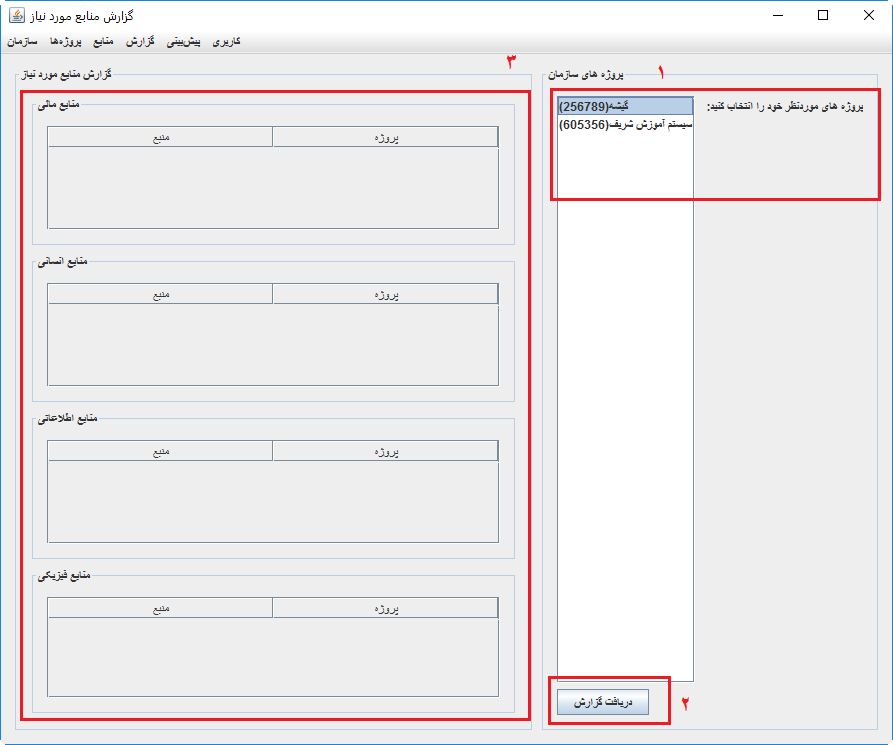
\includegraphics[scale=0.5]{img/manual/reqRep}
		\caption{گزارش منابع موردنیاز}
	\end{figure}
	


\subsection{گزارش جریان چرخشی منابع }
این گزارش چرخش منابع موجود در سازمان را نشان می‌دهد.\\
برای دریافت این گزارش، ابتدا  منابع مدنظر را در بخش ۱ انتخاب نمایید. برای انتخاب چند منبع، کلید Ctrl را نگه داشته و روی منابع مدنظر کلیک کنید. سپس در بخش ۲، یکی از دو حالت بازه‌ی زمانی مشخص یا نامحدود را انتخاب کنید. در صورتی که بازه‌ی زمانی مشخص را انتخاب نمایید، لازم است که ابتدا و انتهای بازه‌ی زمانی مورد نظرتان را نیز وارد نمایید. سپس روی کلید دریافت گزارش (بخش ۳) کلیک کنید تا در بخش ۴ گزارش را مشاهده نمایید.

	\begin{figure}[H]
		\centering
		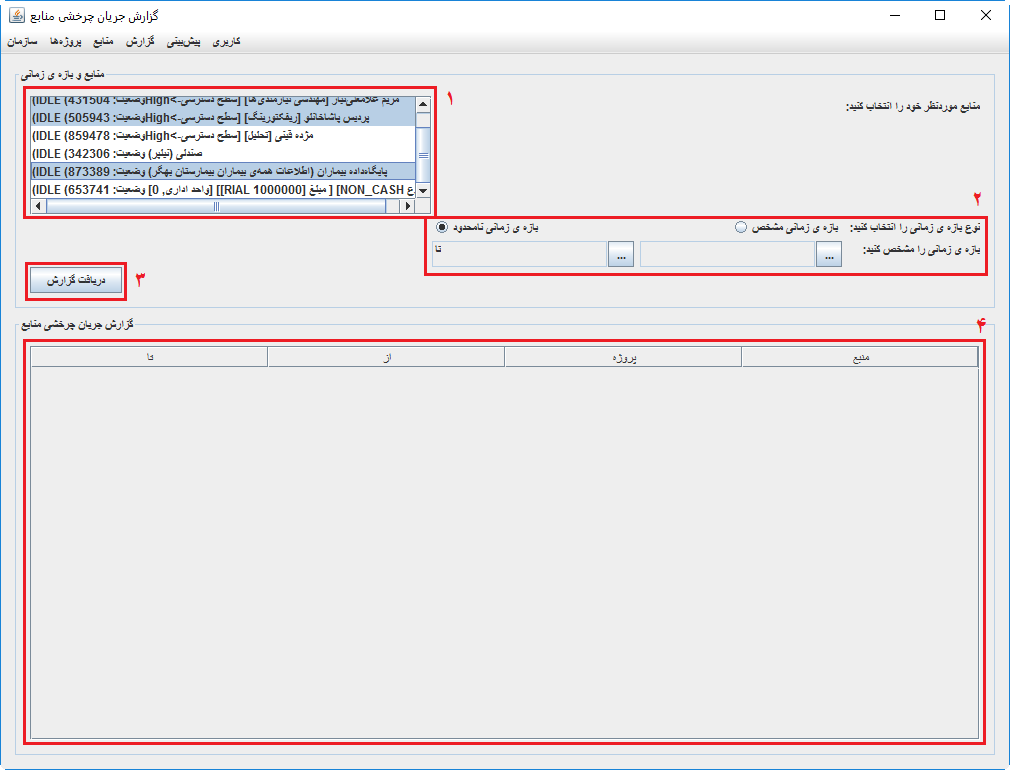
\includegraphics[scale=0.5]{img/manual/flowRep}
		\caption{گزارش جریان چرخشی منابع}
	\end{figure}
	


\newpage
\section{زیرمنوی پیش‌بینی}
این زیرمنو، امکاناتی را برای جستجو در پروژه‌ها و منابع در اختیار مدیران قرار می‌دهد تا مبنای اصلی برای پیش‌بینی‌ها و تصمیم‌گیری‌های دقیق فراهم گردد.
	\begin{figure}[H]
		\centering
		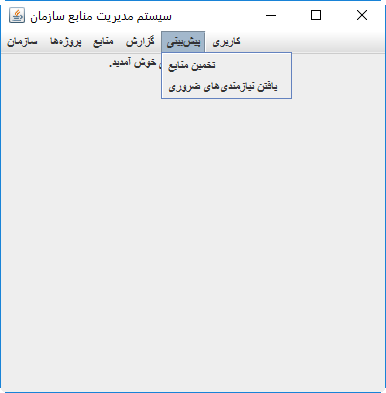
\includegraphics[scale=0.7]{img/manual/estSubmenu}
		\caption{زیرمنوی پیش‌بینی}
	\end{figure}

\subsection{تخمین منابع}
در این بخش ابتدا پارامترهای جستجو که عبارتند از تکنولوژی‌های موردنظر، تعداد توسعه‌دهندگان، تعداد کاربران و تعداد ماژول (۱) تعیین می‌گردند. سپس با فشردن دکمه‌ی جستجو (۲) پروژه‌های مشابه بر اساس پارامترهای تعیین شده آورده می‌شوند(۳).
	\begin{figure}[H]
		\centering
		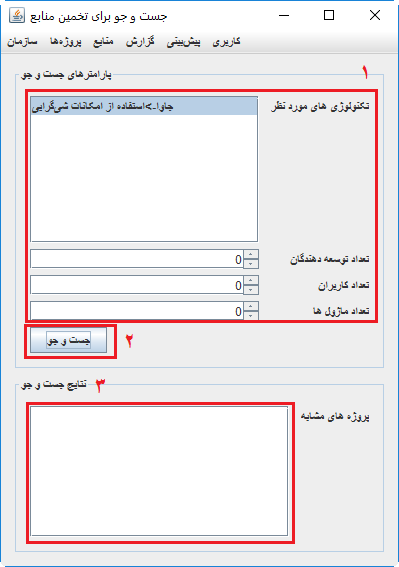
\includegraphics[scale=0.7]{img/manual/searchRes}
		\caption{تخمین منابع}
	\end{figure}

\subsection{یافتن نیازمندی‌های ضروری}
در این بخش، نوع منبع و نام آن (۱) لازم است وارد گردد. سپس با فشردن دکمه‌ی جستجو (۲) منابعی از نوع انتخاب شده که دقیقا نام همسان با نام وارد شده را دارند در بخش ۳ نمایش داده می‌شوند. 

	\begin{figure}[H]
		\centering
		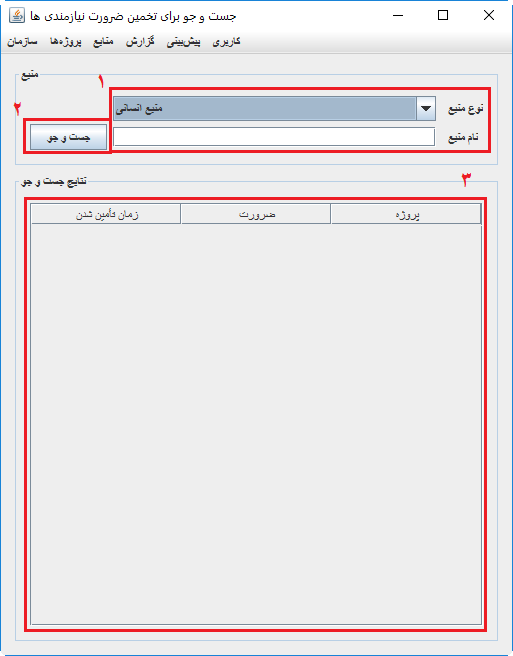
\includegraphics[scale=0.7]{img/manual/estSearch}
		\caption{یافتن نیازمندی‌های ضروری}
	\end{figure}


\newpage
\section{زیرمنوی کاربری}
در این زیرمنو، عملیات مربوط به کاربران قرار دارد.
	\begin{figure}[H]
		\centering
		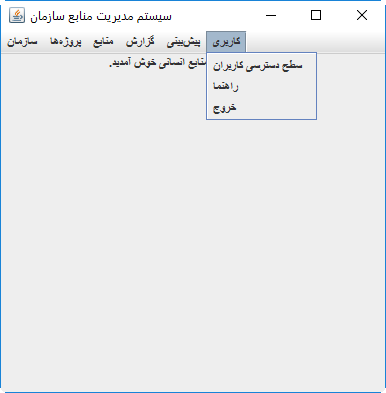
\includegraphics[scale=0.7]{img/manual/userSubmenu}
		\caption{زیرمنوی کاربری}
	\end{figure}

\subsection{سطح دسترسی کاربران}
با انتخاب این گزینه، صفحه‌ای مطابق زیر باز می‌گردد که از طریق آن می‌توان در صورت داشتن اجازه‌ی ویرایش عملیات مجاز سطوح دسترسی، به تغییر عملیات مجاز پرداخت. با گذاشتن یا برداشتن علامت تیک کنار هر یک از موارد (۱) و فشردن دکمه‌ی ذخیره (۲) این تغییرات در سیستم برنامه‌ریزی ثبت می‌گردد.

	\begin{figure}[H]
		\centering
		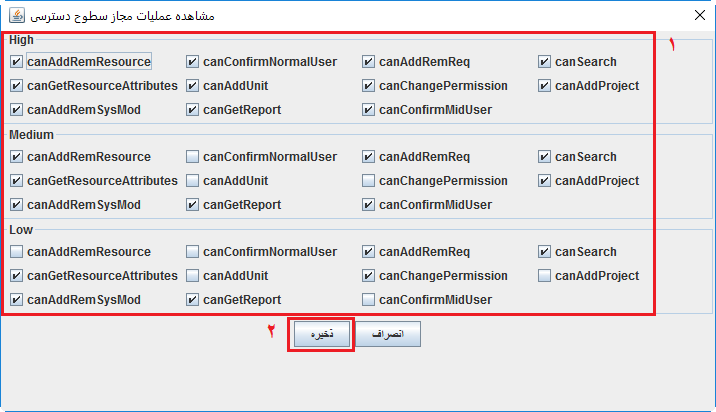
\includegraphics[scale=0.7]{img/manual/ac}
		\caption{سطح دسترسی کاربران}
	\end{figure}

	
\subsection{خروج}
با فشردن این گزینه، کاربر فعلی از سیستم خارج می‌شود و به وی صفحه‌ی ورود به سیستم برنامه‌ریزی نمایش داده خواهد شد.
